\documentclass[12pt,a4paper]{article}%шаблон для статьи, шрифт 12 пт
\usepackage[utf8x]{inputenc} %использование кодировки Юникод UTF-8
\usepackage[russian]{babel} %пакет поддержки русского языка
\usepackage{lipsum}%Рыба-текст
\usepackage[compact]{titlesec}%для titlespacing
\titlespacing*{\section}{0.75cm}{1em}{0.1em}%отступ заголовка
%\titlespacing{\заголовок}{слева}{перед}{после}[справа]
\titlespacing*{\subsection}{0.75cm}{1em}{0.1em}
\usepackage{indentfirst}%отступ первого абзаца
\setlength{\parindent}{0.75cm}
\usepackage[labelsep=endash]{caption}%тире вместо двоеточия в картинках
\usepackage{graphicx}%кртинки
\usepackage{comment}%комментарии
\usepackage{tabularx}%таблицы
\usepackage{amsmath}
\usepackage{amssymb}


%перенос строк внутри таблиц
\newcommand{\specialcell}[2][c]{%
	\begin{tabular}[#1]{@{}c@{}}#2\end{tabular}}

\usepackage[labelsep=endash]{caption} %тире вместо двоеточия в названиях 
%\renewcommand\thefigure{\arabic{section}.\arabic{figure}}
%\renewcommand{\labelenumii}{\arabic{enumi}.\arabic{enumii}.} % Сквозная нумерация

\begin{document}

\thispagestyle{empty}

\begin{center}
\Large{
	\textbf{МИНОБРНАУКИ РОССИИ}
	
	\textbf{Санкт-Петербургский государственный}
	
	\textbf{электротехнический университет «ЛЭТИ»}
	
	\textbf{им. В.И. Ульянова (Ленина)}
	
	\textbf{Кафедра Физики}
}
\end{center}

\topskip=0pt
\vspace*{\fill}
\begin{center}
\Large{
	\textbf{
		ЛАБОРАТОРНАЯ РАБОТА №5(9)\\
		по дисциплине «Физика»\\
		Тема: Исследование термодинамических циклов\\
	}
}
\end{center}
\vspace*{\fill}

\begin{tabular}{lcr}
Студент гр. 9892 & \begin{tabular}{p{60mm}} \\ \hline \end{tabular} & Лескин К.А.  \\\\
Преподаватель    & \begin{tabular}{p{60mm}} \\ \hline \end{tabular} & Чурганова С.С. \\\\
\end{tabular} 

\begin{center}
Санкт-Петербург\\
2020
\end{center}
%////////////////////////////////////////////////////////////////////////////////////////////////
%////////////////////////////////////////////////////////////////////////////////////////////////
%////////////////////////////////////////////////////////////////////////////////////////////////
\newpage

\section*{Цель работы}

Исследование политропно-изохорно-изотермического
($nVT$) и адиабатно-изохорно-изотермического ($SVT$) циклов.

\section*{Приборы и принадлежности}

Баллон с воздухом, манометр, 
микрокомпрессор, лабораторные термометр и барометр.

\section*{Основные исследуемые закономерности}

В лабораторной работе изучаются
политропно-изохорно-изотермический ($nVT$) и адиабатно-изохорно-
изотермический ($SVT$) циклы. В отличие от политропно-изохорно-изотермического цикла в адиабатно-изохорно-
изотермическом цикле процесс расширения газа на участке 1-2* (рис. \ref{pp1}) рассматривается как адиабатический. Изучение циклов
осуществляется путем их моделирования при значениях показателя адиабаты
$ \gamma $=1,4 и показателя политропы n, определенным опытным путем.

\begin{figure}[htp!]
	\centering
	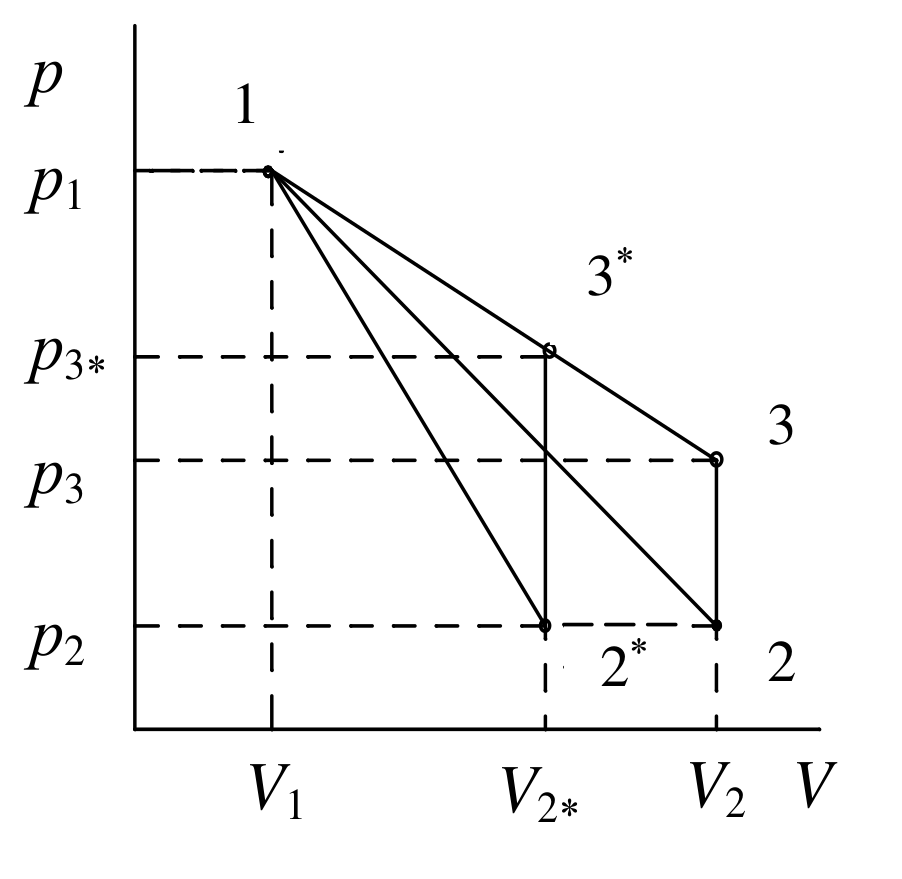
\includegraphics[width=0.7\linewidth]{p1}
	\caption{}
	\label{pp1}
\end{figure}

\newpage

Политропный процесс характерезуется сохранением теплоёмкости газа.

Чтобы определить показатель политропы --- кривой, отображающей изменение состояния газа в политропном процессе --- можно обратиться к первому началу динамики:

\begin{equation}
	\delta Q = dU + \delta A = C_vdT + p dV
\end{equation}

Формулируется он так: сообщённое системе количество теплоты $\delta Q$ расходуется на увеличение внутренней энергии $dU$ системы и
совершение системой работы $\delta А$.

На рис. \ref{pp1} процесс 1-2 является политропным. Телоёмкость $ C $ остаётся постоянной.

Адиабатный процесс происходит без теплообмена с окружающей средой. Он является одним из видов политропных процессов. На рис. \ref{pp1} он соответствует участку 1-2*.

\newpage
\section*{Контрольные вопросы}

\begin{enumerate}
	
	\item Какой газ называют идеальным?
	
	Идеальный газ – это модель разреженного газа, в которой пренебрегается взаимодействием между молекулами, поэтому в объёме, занятом идеальным газом, нет взаимных столкновений частиц. Частицы идеального газа претерпевают столкновения только со стенками сосуда.
	
	\item Дайте определение степеней свободы молекул газа (поступательных, 
	вращательных и колебательных). Как рассчитываются полные степени свободы молекул газа и чему они равны при невысоких температурах для одноатомного, двухатомного и многоатомного газов? Рассчитайте полное число степеней свободы молекул O2 и CO2.
	
	Числом степеней свободы механической системы называется количество независимых величин, с помощью которых может быть задано положение системы. Так, положение в пространстве материальной точки полностью определяется заданием значений трех ее координат, поэтому есть три свободы. Положение абсолютно твердого тела можно определить, задав три координаты его центра инерции $(x,y.z)$. два угла  и , указывающих направление какой-либо оси, связанной с телом и проводящей через его центр инерция, и, наконец, угол, определяющий направление второй связанной с телом оси, перпендикулярной к первой. Таким образам, абсолютно твердое тело имеет шесть степеней свободы. Изменение координат центра инерции при неизменных углах ,  и  обусловливается поступательным движением твердого тела. Поэтому соответствующие степени свободы называются поступательными. Изменение любого из углов (рис. \ref{p1}),  при неизменном положении центра инерции обусловливается вращением тела, в связи с чем соответствующие степени свободы называются вращательными.
	
	\begin{figure}[hpt!]
		\centering
		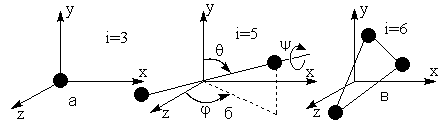
\includegraphics[width=0.5\linewidth]{../lr4(8)/mol}
		\caption{Pавнораспределение энергии по степеням свободы}
		\label{p1}
	\end{figure}
	
	Изменение расстояния между точками соответствует колебанию в системе, поэтому данная степень свободы – колебательная. 
	При определении числа степеней свободы молекулы атомы следует рассматривать как материальные точки.
	
	Для ($O_2$)  $i = 6$.
	
	Для ($CO_2$) $i = 9$.
	
	Одноатомной молекуле нужно приписывать три поступательные степени свободы, двухатомной молекуле, в зависимости от характера связи между атомами, следует приписывать либо три поступательные и две вращательные степени свободы (при жесткой связи), либо, кроме этих пяти, еще одну, колебательную степень свободы (при упругой связи), трехатомной молекуле с жесткой связью – три поступательные, три вращательные, три колебальельные степени свободы. 
	
	\item Какие циклы называют тепловыми, а какие холодильными? 
	Какими параметрами принято характеризовать эффективность этих циклов?
	
	Охлаждение тел до температуры ниже температуры окружающей среды осуществляется с помощью холодильных установок, работающих по обратному тепловому циклу, основные параметры – теплота, отбираемая из холодильного источника, работа в цикле, холодильный коэффициент (чем он выше, тем эффективнее цикл). Если работа положительна, то цикл находится в прямом направлении и называется тепловым, КПД характеризует полезность работы такого цикла (полученная теплота от прохождения цикла).
	
	Работа прямого цикла (за один цикл)
	
	\begin{equation}
	A = Q_1 - Q_2
	\end{equation}
	
	$Q_1$ --- полученное количество теплоты от нагревания.
	
	$Q_2$ --- отданное количество теплоты холодильнику.
	
	КПД $\eta$
	
	\begin{equation}
	\eta = \dfrac{A}{Q_1}
	\end{equation}
	
	Работа холодильной машины (за один цикл)
	
	\begin{equation}
	A = Q_2 - Q_1
	\end{equation}
	
	$Q_1$ --- полученное количество теплоты от холодильника.
	
	$Q_2$ --- отданное количество теплоты нагревателю.
	
	КПД $\eta$
	
	\begin{equation}
	\eta = \dfrac{Q_1}{A}
	\end{equation}
	
	\item Что такое состояние вещества? Какие величины
	называют параметрами состояния? Напишите уравнение состояния идеального газа.
	
	Состояние вещества зависит от сочетания температуры и давления, это физическое состояние вещества. Параметры состояния включают в себя форму, плотность, скачкообразность изменения свободной энергии, энтропии. Например, уравнение состояния идеального газа показывает зависимость между давлением, абсолютной температурой идеального газа и его молярным объемом: $pV_m = RT$
	или $pV = vRT$, где $p$ – давление, $V$ – объем газа ($V_m$ – молярный объем), $v$ – количество газа, $R$ – универсальная постоянная, $T$ – термодинамическая температура, К. 
	
	\item Дайте определение термодинамических функций: работы газа $A$, его
	внутренней энергии $U$, количества теплоты $Q$, отдаваемой (получаемой) газом, энтропии $S$ . Какие из этих функций являются функциями состояния, а какие функциями процесса? Чему равно изменение функций состояния в цикле?
	
	Под работой $A$ в термодинамике, в зависимости от контекста, понимают как действие обмена энергией между термодинамической системой и окружающей средой, не связанное с переносом вещества и/или теплообменом (работа как способ/форма передачи энергии, работа как форма обмена энергией, работа как особый вид энергии в процессе перехода, то есть как функционал процесса, «не существующий» до процесса, после процесса и вне процесса), так и количественную меру этого действия, то есть величину передаваемой энергии. Эта функция процесса, так же как и количество теплоты. Внутренняя энергия газа определяется как сумма потенциальной и кинетической энергии, и является функцией состояния. Изменение функций состояния в любом термодинамическом процессе равно разности её значений в конце и в начале процесса и не зависит от пути процесса. Энтропия (функция состояния) – в состоянии термодинамического равновесия она достигает максимума, ее изменение в любом циклическом процессе равно $0$. Количество теплоты подразумевается, как энергия, переданная телу в результате теплообмена (теплоемкость), описывает функцию процесса. 
	
	\item Какие процессы называют политропными? Дайте определение показателя политропы.
	Чему равны показатели политропы для изохорного, изобарного, изотермического и адиабатного процессов? 
	
	Политропные процессы - термодинамический процесс, во время которого теплоёмкость газа остаётся неизменной. Политропа отображает данные процессы на кривой на термодинамических диаграммах. На рис. \ref{p2} показана таблица для показателя политропы в различных термодинамических процессах, исходя из уравнения политропы для идеального газа: $PV^n = const$
	, где произведение давления и объема в степени политропы является константным значением. 
	
	\begin{figure}[hpt!]
		\centering
		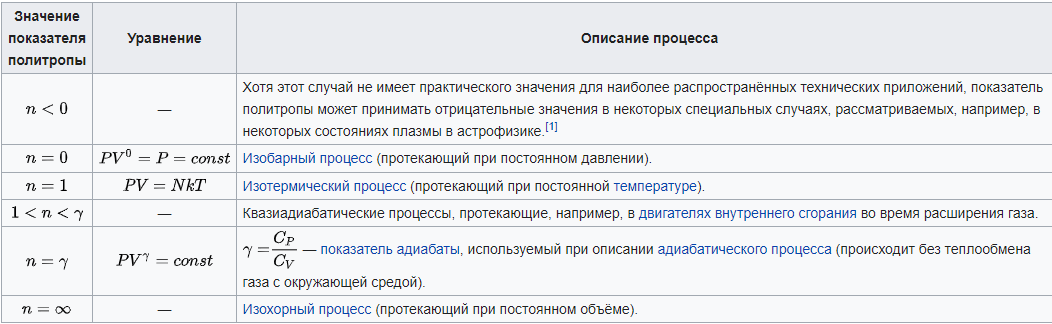
\includegraphics[width=\linewidth]{p2}
		\caption{Pазличные значения показателя политропы}
		\label{p2}
	\end{figure}
	
	
	\item Как экспериментально определяется показатель политропы в данной работе? Докажите формулу, по которой он рассчитывается.
	
	Процесс расширения воздуха на участке 1-2 (рис. \ref{p3}) является политропным, в котором теплоёмкость газа $С$ остаётся постоянной. Первое начало термодинамики для политропного процесса имеет вид:$CdT = C_vdT+pdV$, где $С$ – теплоемкость воздуха в политропном процессе. Из этого соотношения с помощью уравнения состояния идеального газа можно получить уравнение Пуассона для политропного процесса $TV^{n-1}$, где $n$ – показатель политропы, в таком случае, $n = \dfrac{C_p - C}{C_v - C}$
	, где $C_p$ и $C_v$ – теплоемкость газа в изобарном и изохорном процессах.
	
	\begin{figure}[hpt!]
		\centering
		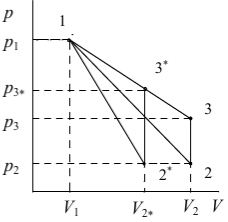
\includegraphics[width=0.5\linewidth]{p3}
		\caption{Показатели давления воздуха и его объема в баллоне}
		\label{p3}
	\end{figure}
	
	Предположим, что процесс расширения воздуха на участке 1-2* (рис. \ref{p3}) является адиабатным. Адиабатный процесс является одним из видов политропных процессов, он происходит без теплообмена с окружающей средой, и теплоемкость газа в этом процессе $С=0$. Поэтому показатель политропы в этом процессе равен омеге и называется показателем адиабаты. Взаимосвязь между параметрами состояния в адиабатном процессе также описывается уравнениями Пуассона либо объединенным газовым законом. Показатель политропы $n$ может быть определён экспериментально. Выразим $n$ через экспериментально измеряемые велечины, для чего продифференцируем уравнения политропы ($pVn = const$) и изотермы ($pV = const$): $pnV^{n-1}dV + V^nd_p = 0$ – для политропы и $pdV+Vd_p = 0$ – для изотермы. Выразим одно через другое, вычислим угловые коэффициенты политропы 1-2 и изотерма 1-3 (см. рис. 3), получаем показатель политропы $n = \dfrac{\Delta_{p_{1}}}{\Delta_{p_{1}}-\Delta_{p_{3}}}$.
	
	\item  Сформулируйте объединенный газовый закон, и, исходя из него, напишите уравнения изохоры, изобары и изотермы.
	
	Объединенный газовый закон позволяет вычислить объем газ при определенной температуре и давлении, если известен его объем при других значениях температуры и давления. Объединяя законы Бойля-Мариотта и Гей-Люссака, получаем уравнение $\dfrac{p_1v_1}{T_1} = \dfrac{p_2v_2}{T_2}$ ($p$ – давление, $V$ – объем), которое является математическим выражением объединенного газового закона. Его другая форма написания: $\dfrac{pv}{T} = const$. Исходя из него, уравнения изохоры: $\dfrac{p_1}{T_1} = \dfrac{p_2}{T_2}$, уравнение изобары --- $\dfrac{V_1}{T_1} = \dfrac{V_2}{T_2}$, уравнение изометры --- $P_1V_1 = P_2V_2$.
	
	\item Сформулируйте первое начало термодинамики. Какой вид оно имеет
	для каждой из ветвей цикла, а также всего цикла? Напишите первое начало для изобарного, изохорного, изотермического и адиабатного процессов.
	
	Первый закон термодинамики является обобщением закона сохранения и превращения энергии для термодинамической системы. Он формулируется следующим образом: изменение $\Delta U$ внутренней энергии неизолированной термодинамической системы равно разности между количеством теплоты $Q$, переданной системе, и работой $A$, совершенной системой над внешними телами: $\Delta U = Q - A$. Согласно этому закону, энергия не может быть создана или уничтожена; она передается от одной системы к другой и превращается из одной формы в другую.
	В изохорном процессе ($V=const$) газ работы не совершает, $A=0$. Следовательно, $Q = \Delta U = U(T_2) - U(T_1)$ Здесь $U(T_2)$ и $U(T_1)$ – внутренние энергии газа в начальном и конечном состояниях. Внутренняя энергия идеального газа зависит только от температуры (закон Джоуля). При изохорном нагревании тепло поглощается газом ($Q>0$), и его внутренняя энергия увеличивается. При охлаждении тепло отдается внешним телам ($Q<0$).
	
	В изобарном процессе ($p=const$) работа, совершаемая газом, выражается соотношением $A = p(V_2-V_1) = p\Delta V$  Первый закон термодинамики для изобарного процесса дает: $Q = U(T_2) - U(T_1) + p(V_2-V_1) = \Delta U + p\Delta V$. При изобарном расширении $Q>0$ – тепло поглощается газом, и газ совершает положительную работу. При изобарном сжатии $Q<0$ – тепло отдается внешним телам. В этом случае $A<0$. Температура газа при изобарном сжатии уменьшается, $T_2 < T_1$; внутренняя энергия убывает, $\Delta U < 0$.
	
	В изотермическом процессе температура газа не изменяется, следовательно, не изменяется и внутренняя энергия газа $\Delta U = 0$. Первый закон термодинамики для изотермического процесса выражается соотношением $Q=A$.
	
	Количество теплоты $Q$, полученной газом в процессе изотермического расширения, превращается в работу над внешними телами. При изотермическом сжатии работа внешних сил, произведенная над газом, превращается в тепло, которое передается окружающим телам.
	
	\item Дайте определение удельной и мольной теплоемкостей вещества. Как они взаимосвязаны друг с другом? Каковы их размерности?
	
	Если в результате теплообмена телу передается некоторое количество теплоты, то внутренняя энергия тела и его температура изменяются. Количество теплоты $Q$, необходимое для нагревания 1 кг вещества на 1 К называют удельной теплоемкостью вещества $c = \dfrac{Q}{m\Delta T}$
	Во многих случаях удобно использовать молярную теплоемкость $C = M c$, где $M$ – молярная масса вещества. При нагревании жидких и твердых тел их объем практически не изменяется, и работа расширения оказывается равной нулю. Поэтому все количество теплоты, полученное телом, идет на изменение его внутренней энергии. В отличие от жидкостей и твердых тел, газ в процессе теплопередачи может сильно изменять свой объем и совершать работу. Поэтому теплоемкость газообразного вещества зависит от характера термодинамического процесса. Обычно рассматриваются два значения теплоемкости газов: $C_v$ – молярная теплоемкость в изохорном процессе ($V = const$) и $C_p$ – молярная теплоемкость в изобарном процессе ($p = const$). Отношение теплоемкостей в процессах с постоянным давлением и постоянным объемом играет важную роль в термодинамике. Оно обозначается греческой буквой $\gamma$.
	
	\item Как можно вычислить теплоемкость идеального газа в произвольном 
	политропном процессе через показатель политропы? Докажите эту формулу.
	
	Так как в ответе на вопрос седьмой я выразил политропу, ее можно использовать для вычисления теплоемкости идеального газа. Зная $n$, можно определить мольную теплоемкость газа в политропном процессе (мольные величины обозначаем соответствующими строчными буквами): $c = c_v\dfrac{n - \gamma}{n-1}$, где $\gamma$ равна отношению теплоемкостей газа в изобарном и изохорном процессе (показатель адиабаты). $ c_v = \dfrac{iR}{2} $, $ c_p = c_v+R = \dfrac{(i+2)R}{2} $ , где $i$ число степеней свободы молекул газа, $R$ – универсальная газовая постоянная. 
	
	
	\item Объясните, почему теплоемкость воздуха в политропном процессе в данной работе отрицательна?
	
	Отрицательную теплоемкость газа в данной работе можно объяснить с помощью рисунка \ref{p3}, так как на участке 1-2 воздух охлаждается, а тепло через стеклянную колбу поступает в систему ($ dQ>0, dT<0 $) поэтому теплопоемкость газа в политропном процессе $ c = \dfrac{dQ}{dT} $ – отрицательна.
	
	\item Напишите уравнение Пуассона в переменных (p,V), (p,T) и (V,T).
	
	Само уравнение Пуассона в адиабатном процессе принято записывать, как: 
	$ PV^k = const $
	Здесь $V$ – объем, занимаемый газом, $P$ – его давление, а велечина $k$ называется показателем адиабаты, так описываются переменные $p$ и $V$. С помощью уравнения Клапейрона-Менделеева уравнение можно переписать, используя другие параметры состояния идеального газа (другие переменные): 
	$ TV^{y-1} = const $
	, 
	$ P^{1-y}T^{y-1} = const $ .
	
	\item Дайте определение холодильного коэффициента. Как он вычисляется в цикле, изучаемом в данной работе?
	
	Холодильный коэффициент характеризует эффективность холодильного (против часовой стрелки) цикла, он определяется как отношение теплоты, отнятой от охлаждаемого газа, к затраченной в цикле работе. 
	
	\begin{equation}
	\eta = \dfrac{Q_1}{A} = \dfrac{Q_1}{Q_2 - Q_1}
	\end{equation}
	
	$Q_1$ --- полученное количество теплоты от холодильника.
	
	$Q_2$ --- отданное количество теплоты нагревателю.
	
	\item Как соотносятся холодильные коэффициенты $nVT-$ и $SVT-$ циклов? Какой из них больше и почему?
	
	Для $SVT-$цикла с учетом $Q_{12}=0$ и $Q_{23}|\Delta U_{23}|=|\Delta U_{12}|= A_{12}$ холодильный коэффициент $ \varepsilon (SVT) = \dfrac{A_{12}}{A_{13} - A_{12}} $ , а для $nVT-$цикла в предположении $Q_{12}$ примерно равен 0: $ \varepsilon (nVT) = \dfrac{A_{12}}{A_{13} - A_{12}} $ . Отношение холодильных коэффициентов $ \dfrac{\varepsilon(nVT)}{\varepsilon (SVT)} > 1 $
	
	\item Покажите, что холодильный коэффициент (ХК)  холодильника и КПД тепловой машины, работающих по взаимно обратным циклам, связаны соотношением $ \varepsilon = \dfrac{1}{\eta-1}$.
	
	Из опредения коэффициента полезного действия во всех случаях должен быть правильной дробью как отношение полезного эффекта к энергетическим затратам. Тепловые насосы, работающие по обратным циклам, позволяют осуществить перенос теплоты от холодных тел к горячим. Коэффициент полезного действия для тепловых машин следует определить как отношение разницы поступающей в рабочее тело энергии и энергии компенсации к энергии. Так как термический КПД произвольного прямого цикла $ y\eta = \dfrac{Q_1 - Q_2}{Q_1} $, то $ \psi = \dfrac{1}{y\eta} $. Из второй теоремы Карно получается $ \dfrac{1}{\psi c} $ или $ \psi c < psi $. Таким образом, любой обратный цикл при заданных пределах температур имеет отопительный коэффициент выше, чем соответствующий цикл Карно. Тот же результат можно получить, сравнивая цикл Карно и произвольный обратный цикл на B, T-диаграмме. Сопоставляемые циклы должны располагаться между предельными температурами T1 и T2, чтобы исключить неоднозначность.
	
	\item В каких интервалах изменяются ХК $\varepsilon$ и КПД $ \eta $? Может ли тепловая
	машина с высоким КПД, если ее цикл обратить, работать как хороший холодильник, и наоборот?
	
	Холодильная машина может отвести от охлаждаемого конца больше теплоты, чем затрачивается энергии на организацию процесса. Эффективность машин характеризует холодильный коэффициент ХК. Наилучшими показателями производительности для холодильных машин обладает обратный цикл Карно: в нём холодильный коэффициент зависит от температур горячего и холодного концов. 
	
	Данная велечина, очевидно, может быть сколь угодно велика; хотя практически к ней трудно приблизиться, холодильный коэффициент может превосходить единицу. Это не противоречит первому началу термодинамики, поскольку, кроме принимаемой в расчёт энергии $A$ (напр., электрической), в тепло $Q$ идёт и энергия, отбираемая от холодного источника.
	
	\item Дайте термодинамическое и статистическое (формула Больцмана) определение энтропии. Как можно вычислить ее изменение в произвольном политропном процессе?
	
	Функция состояния, дифференциалом которой является отношение $\dfrac{\delta Q}{T}$, называется энтропией
	
	\begin{equation}
	dS = \dfrac{\delta Q}{T}, \varDelta S = \int_1^2{ \dfrac{\delta Q}{T}} = vc\int_1^2 \dfrac{dT}{T} = vc\ln{\dfrac{T_2}{T_1}}
	\end{equation}

	Здесь $c$ - мольная теплоемкость газа, зависящая от типа политропного процесса (адиабатный, изохорный, изобарный и т.п.). Отметим, что данное выражение справедливо лишь для обратимых процессов, то есть процессов, которые могут быть проведены в обратном направлении через те же промежуточные состояния, что и при прямом процессе; при этом тепловое состояние окружающей среды не изменяется (процесс без теплопотерь). 
	
	Выразим изменение энтропии $ \Delta S $ через экспериментально определяемые
	в опыте величины давлений сначала для $nVT-$цикла. В политропном процессе
	(на участке 12, рис. \ref{p3}) с учетом уравнения Пуассона для переменных $T, p$  получим: 
	
	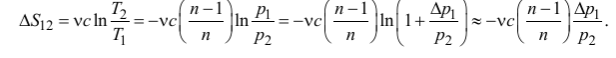
\includegraphics[width=\linewidth]{p5}

	
	\item Какие формулировки второго начала термодинамики вам известны? Дайте энтропийную формулировку второго начала.
	
	Вот некоторые формулировки второго начала термодинамики: 
	
	Теплота не может самопроизвольно переходить от менее нагретого тела к более нагретому (постулат Клаузиуса); 
	
	Невозможен процесс, единственным результатом которого является превращение теплоты в работу; 
	
	Невозможно построить машину, все действия которой сводились бы к производству работы за счет охлаждения теплового источника (вечный двигатель второго рода); 
	
	Любая форма энергии может полностью перейти в теплоту, но теплота преобразуется в другие формы энергии лишь частично; 
	
	В изолированных системах самопроизвольно могут протекать только процессы, сопровождающиеся увеличением энтропии; 
	
	Энтропия изолированной системы не может самопроизвольно убывать.
	
\end{enumerate}
\end{document}